% %---------------------导言区---------------------------%
\documentclass[12pt,a4paper,UTF8]{ctexart}
\usepackage{geometry}
	\geometry{left=2.5cm,right=2.5cm,top=3.2cm,bottom=2.8cm}
\usepackage{xeCJK,amsmath,paralist,enumitem,booktabs,multirow,graphicx,subfig,setspace,listings,lastpage}
\usepackage[colorlinks,
            linkcolor=blue,       
            anchorcolor=blue,  
            citecolor=blue,       
            ]{hyperref}
	\setlength{\parindent}{2em}
	\lstset{language=Python}
\usepackage{fancyhdr}
	\pagestyle{fancy}
	\rhead{B6/B14 交流电桥测电感电容及Multisim电路仿真}
	\lhead{基础物理实验\uppercase\expandafter{\romannumeral2}补充材料}
	\cfoot{Page \thepage/\pageref{LastPage}}  %当前页\总页数
	\rfoot{\today}
	\renewcommand{\headrulewidth}{0.4pt}
	\renewcommand{\theenumi}{(\arabic{enumi})}

\renewcommand{\thefigure}{S\arabic{figure}}
\renewcommand{\thetable}{S\arabic{table}}
%%%%%%%%%%%%%%%%%%%%%%%%%%%%%%%%%%%%%%%%%%%%%%%%%%%%%%%%%%
%%%%%%%%%%%%%%%%%%%%%%%%%正文开始%%%%%%%%%%%%%%%%%%%%%%%%%%
%%%%%%%%%%%%%%%%%%%%%%%%%%%%%%%%%%%%%%%%%%%%%%%%%%%%%%%%%%

\begin{document}

\begin{center}
\LARGE\textbf{B6/B14 交流电桥测电感电容及Multisim电路仿真实验 补充材料}
\end{center}

%%信息
\begin{doublespacing}
	\centering
	\begin{tabular}{ll}
	 & \\
	{\CJKfontspec{Droid Sans Fallback} 实验人:黄子维 20980066} & {\CJKfontspec{Droid Sans Fallback}合作者:黄睿杰 20980062}\\
	{\CJKfontspec{Droid Sans Fallback} 实验时间:2021.11.18~星期四~上午} & {\CJKfontspec{Droid Sans Fallback} 室温:21$^{\circ}$C~相对湿度:35\%}
	\end{tabular}
\end{doublespacing}


\subsection*{实验设备}
\begin{table}[htbp]
    \centering
        \begin{tabular}{cccc}
            \toprule
            编号 &名称 &数量 &仪器参数及型号 \\
            \midrule
            1	&$NI-VisualBench$一体化仪器	&1	&$VB-8012$    \\    
            2	&实验测控用计算机	&1	&$ideaCENTER-B320i$   \\
            3	&标准电容$C_0$	&1	&$0.47 \mu F$ \\
            4	&标准电阻$R_2$	&1	&$510 \Omega$   \\
            5	&电阻箱	&2	&$FBZX21Z$    \\
            6	&数字电桥	&1	&$TH2811D$    \\
            7   &Multisim平台   &1  &$Multisim 12.0$  \\
            8   &黑箱电路   &1  &$\#7$    \\
            \bottomrule
        \end{tabular}
        \caption{\textbf{实验设备}}
\end{table}	

\subsection*{交流电桥实验参数}

\begin{table}[htbp]
    \centering
        \begin{tabular}{cc}
            \toprule
            元件 &参数  \\
            \midrule
            R2(R3) &510$\Omega$ \\
            $C_0$ &0.47$\mu F$ \\
            $\omega_0$ &10$kHz$ \\
            \bottomrule
        \end{tabular}
        \caption{\textbf{交流电桥实验参数}}
\end{table}	

\subsection*{电容和电感测量不确定度}
结果分别如表\ref{tab:1.1}和表\ref{tab:1.2}
\begin{table}[htbp]
	\centering
	\begin{minipage}{0.45\linewidth}
		\begin{tabular}{cccc}
            \toprule
            参数 &$S_A$ &$S_B$ &$S$   \\
            \midrule
            $C_x/ nF$    &0.387   &0.0532  &0.391 \\
            $r_C/ \Omega$   &0.47   &0.22   &0.52 \\
            $Z_C/ \Omega$   &0.45   &0.09   &0.47 \\
            $D$             &0.003  &0.001  &0.004 \\
            \bottomrule
        \end{tabular}
        \caption{\textbf{电容测量不确定度}}
		\label{tab:1.1}
	\end{minipage}
	\begin{minipage}{0.45\linewidth}
		\begin{tabular}{cccc}
            \toprule
            参数 &$S_A$ &$S_B$ &$S$   \\
            \midrule
            $L_x/ mH$    &0.586  &0.01   &0.586 \\
            $r_L/ \Omega$   &2.97   &0.07   &2.97 \\
            $Z_L/ \Omega$   &36.96   &0.87   &36.97 \\
            $Q$             &0.002  &0.002  &0.003 \\
            \bottomrule
        \end{tabular}
        \caption{\textbf{电感测量不确定度}}
        \label{tab:1.2}
	\end{minipage}
\end{table}

\subsection*{仿真实验}
\subsubsection*{RLC仿真}
RLC,RC,RL仿真电路图分别如图\ref{fig:1.1},图\ref{fig:1.2}和图\ref{fig:1.3}所示。
\begin{figure}[htbp]
    \centering
    \subfloat[RLC电路]{\label{fig:1.1}
    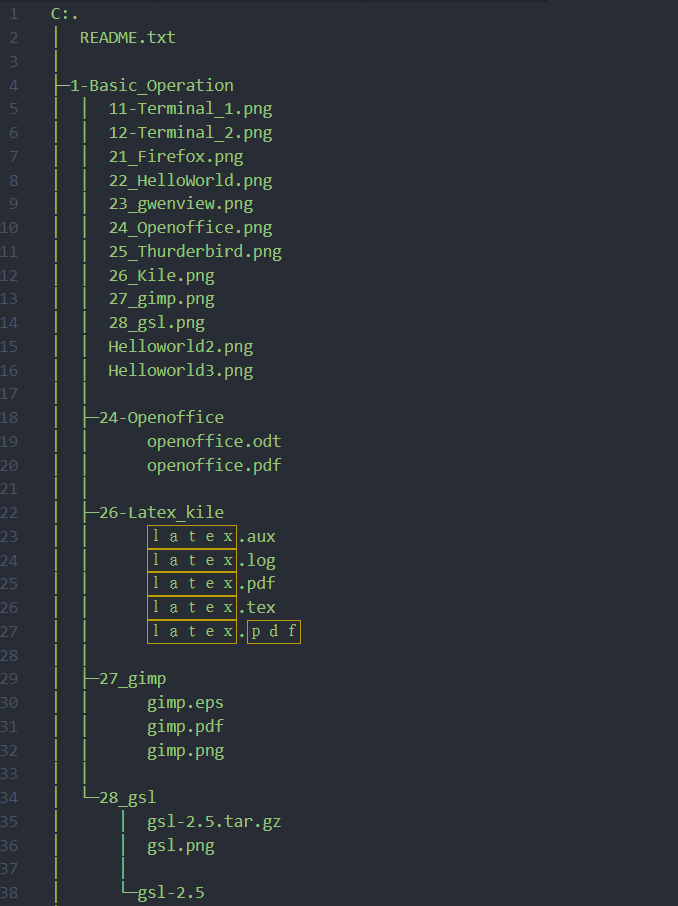
\includegraphics[width=0.3\textwidth]{attachments/fig.s1.1.png}
    }
    \subfloat[RC电路]{\label{fig:1.2}
    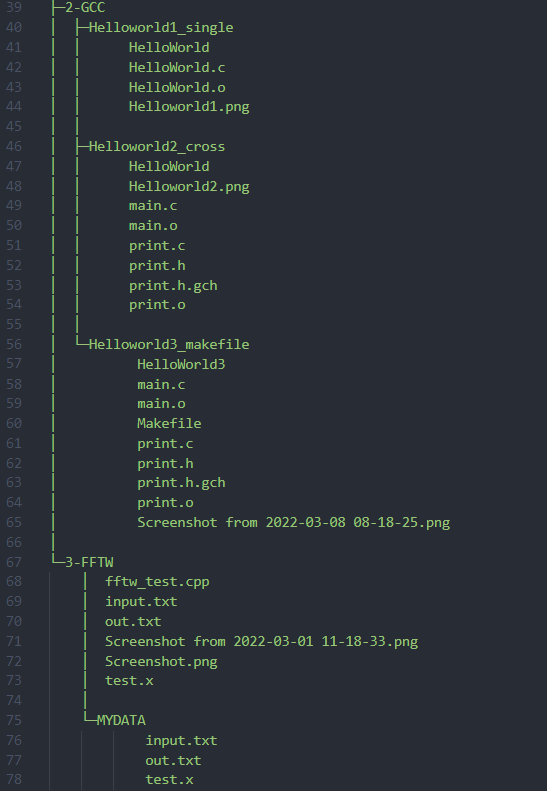
\includegraphics[width=0.3\textwidth]{attachments/fig.s1.2.png}
    }
    \subfloat[RL电路]{\label{fig:1.3}
    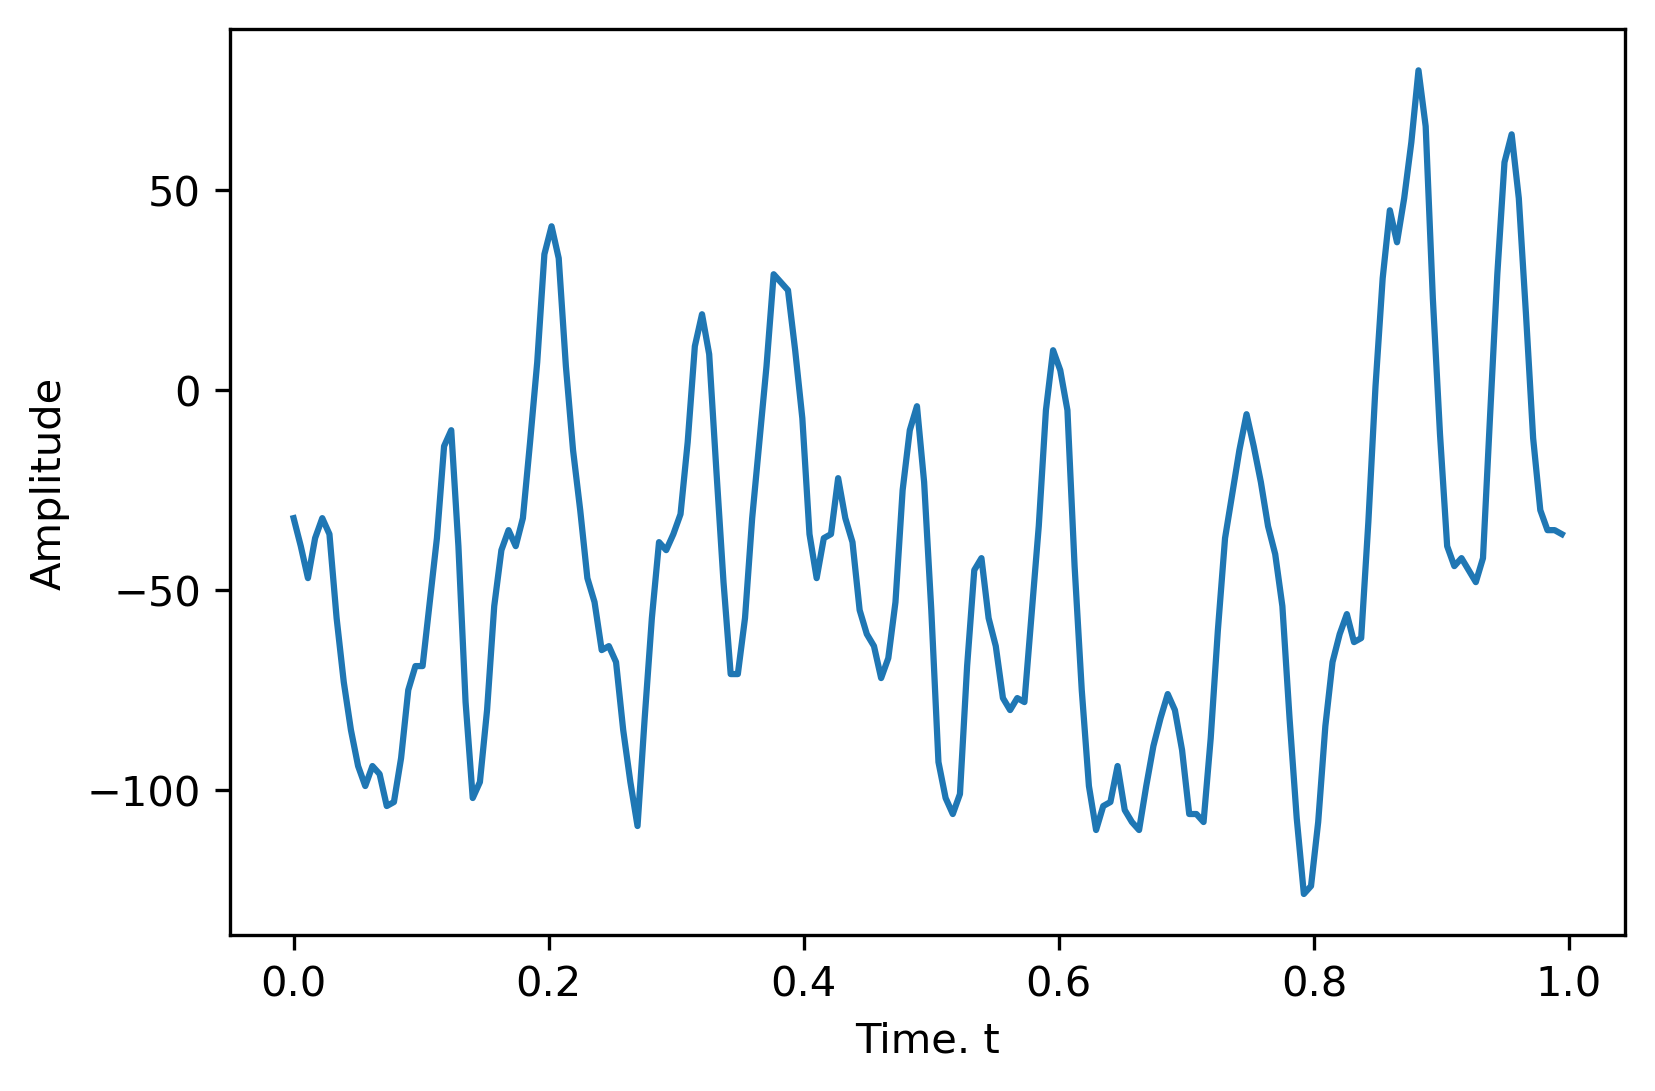
\includegraphics[width=0.3\textwidth]{attachments/fig.s1.3.png}
    }
    \caption{RLC仿真}
\end{figure}
\subsubsection*{非直流电桥实验}
实验结果如图\ref{fig:2}
\begin{figure}[htbp]
    \centering
    \subfloat[0mV]{
    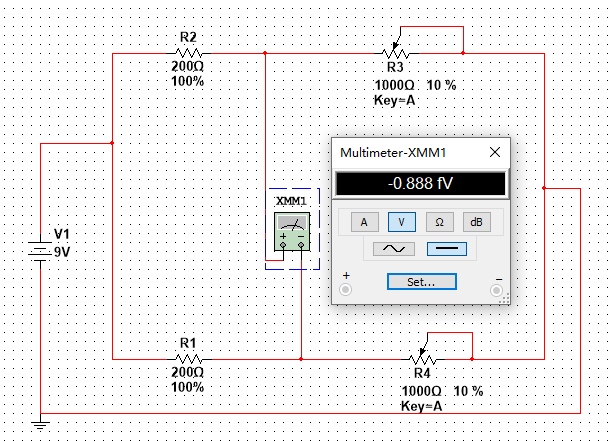
\includegraphics[width=0.25\textwidth]{attachments/fig.s2.1.png}
    }
    \subfloat[10mV]{
    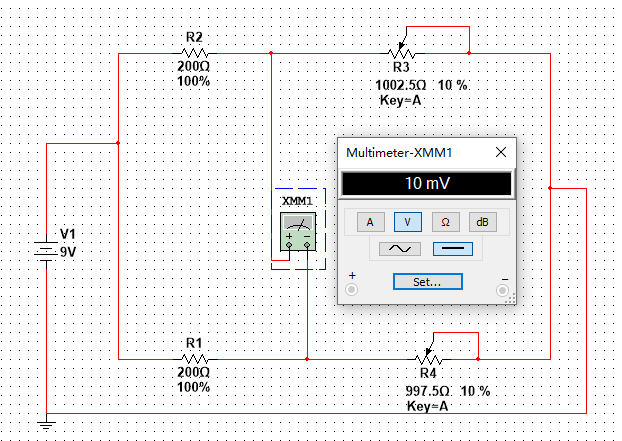
\includegraphics[width=0.25\textwidth]{attachments/fig.s2.2.png}
    }

    \subfloat[20mV]{
    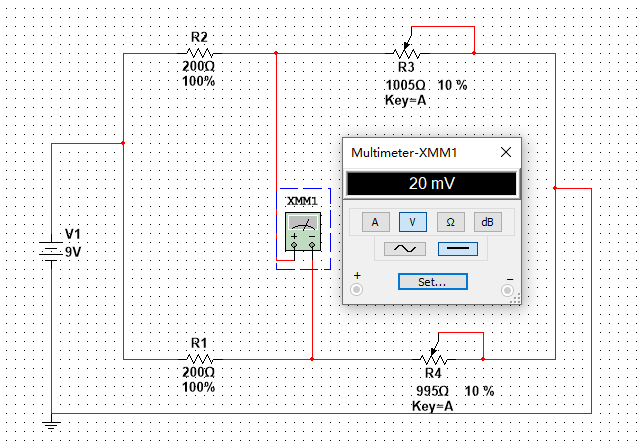
\includegraphics[width=0.25\textwidth]{attachments/fig.s2.3.png}
    }
    \subfloat[30mV]{
    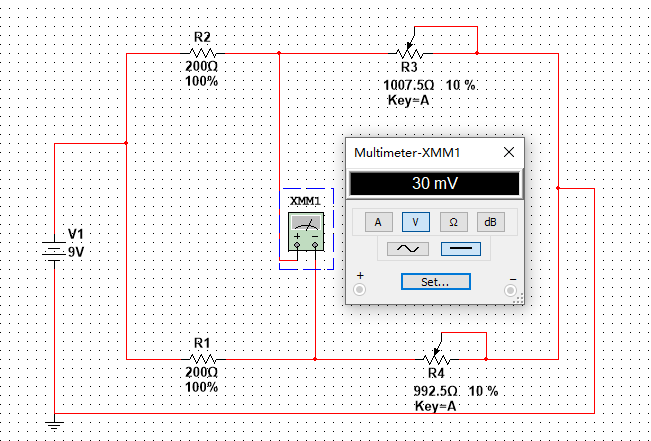
\includegraphics[width=0.25\textwidth]{attachments/fig.s2.4.png}
    }
    \subfloat[40mV]{
    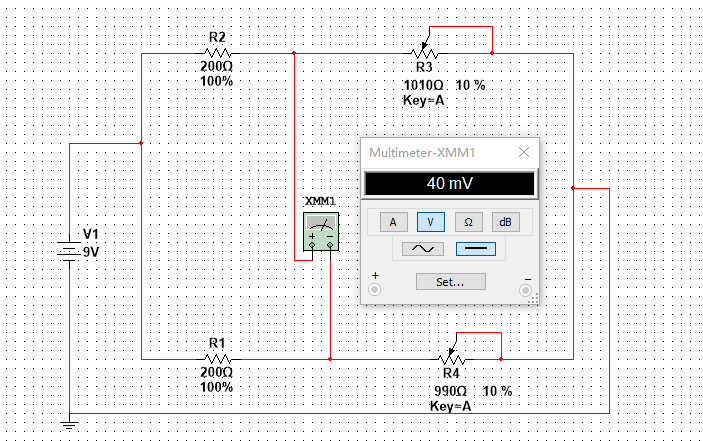
\includegraphics[width=0.25\textwidth]{attachments/fig.s2.5.png}
    }
    \caption{非直流电桥}
    \label{fig:2}
\end{figure}

\subsubsection*{交流电桥}
结果如图\ref{fig:3}
\begin{figure}[htbp]
    \centering
    \subfloat[电容电桥]{
    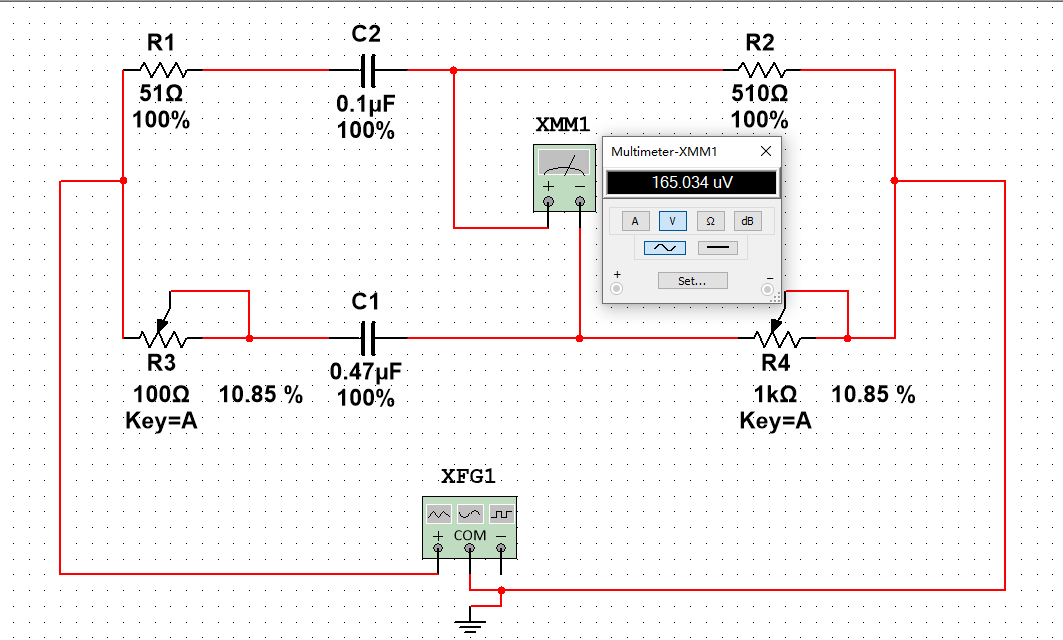
\includegraphics[width=0.4\textwidth]{attachments/fig.s3.1.png}
    }
    \subfloat[电感电桥]{
    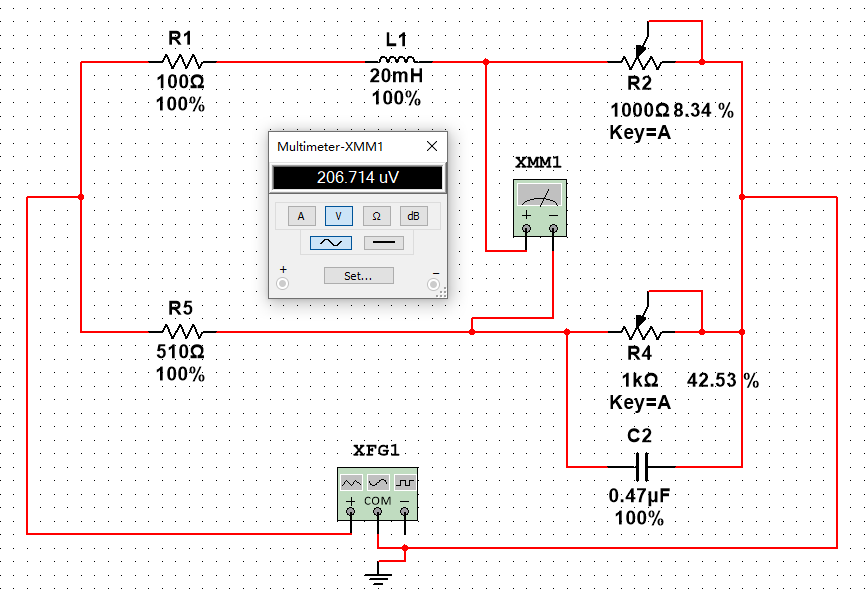
\includegraphics[width=0.4\textwidth]{attachments/fig.s3.2.png}
    }
    \caption{交流电桥}
    \label{fig:3}
\end{figure}

\subsection*{思考题}
\subsubsection*{1. 交流电桥和直流电桥有何区别?}
交流电桥中包含电阻、电感、电容等电路元件,交流电桥平衡时,除相对两臂交流阻抗的模的乘积相等外,
阻抗的相位角还需要满足相对两臂相位角之和相等。而直流电桥只含有纯电阻元件,电桥平衡只要求相对两臂阻值乘积相等。
\subsubsection*{2. 麦克斯威尔-维恩电桥中,R0和C0组成的桥臂若改成串联形式,电桥是否还能达到平衡?比较这两种形式的电桥,哪一种电桥适合测量高Q值的电感,那一种适合测量低Q值的电感?}
\begin{enumerate}[label=\arabic*.]
    \item 改成串联之后电路仍可满足电桥平衡条件,电桥仍可平衡。
    \item 串联状态下电桥更适合用于测高 Q 值电感,并联状态下的电桥更适合用于测低 Q 值电感。
    \item 原因为:串联状态下,电阻和电容的总阻抗最大值较大,并联状态下较小。若要测 Q 较大的电感(内阻较小),则所需的总阻抗应较大,应当选择串联。反之则应选择总阻抗较小的方式,即并联。
\end{enumerate}
\subsubsection*{3. 分析下列四种电桥线路是否能实现平衡,为什么?}
\begin{enumerate}[label=\arabic*.]
    \item (a) 为麦克斯韦尔-维恩电桥,可以平衡
    \item (b) 相邻两臂为纯电阻,另外两臂不同为电感或电容,无法满足相位平衡条件,因此不能平衡
    \item (c) 相对两臂为纯电阻,另外两臂不分别为电容和电感,无法满足相位平衡条件,因此不能平衡
    \item (d) 相邻两臂为纯电阻,另外两臂同为电容,因此能平衡
\end{enumerate}
\subsubsection*{4. 推导直流电桥中1/4桥、半桥、全桥的输出电压与桥臂电阻之间的对应公式。}
电桥不平衡时,AB两点电压$\Delta U$
\begin{equation}
    \Delta U = \frac{R_1R_4-R_3R_2}{(R_1+R_2)(R_3+R_4)}U
\end{equation}
四分之一桥
\begin{gather}
    R_1=R_2=R_3=R   \\
    R_4 = R' + \Delta R \\
    \Delta U = \frac{R'- R + \Delta R}{2(R'+ R + \Delta R)}U
\end{gather}
半桥
\begin{gather}
    R_1=R_3=R   \\
    R_2 = R' + \Delta R \\
    R_4 = R' - \Delta R \\
    \Delta U = \frac{-2R\Delta R}{(R'+ R)^2 - (\Delta R)^2)}U
\end{gather}
全桥
\begin{gather}
    R_1=R_4=R - \Delta R    \\
    R_2=R_3=R + \Delta R    \\
    \Delta U = \frac{-\Delta R}{R}U
\end{gather}

\subsection*{项目源码}
\href{https://github.com/Jeg-Vet/SYSU-PHY-EXP/tree/main/B6-AC_bridge}{SYSU-PHY-EXP/B6 AC bridge.Jeg-Vet(github.com)}

\end{document}